\section{Concept selection}\label{cha:conceptselection}
This chapter describes the steps leading up to the selection of the stacked toroid configuration. The stacked toroid concept has been found to yield the most favourable combination of characteristics and thereby selected by the customer for further analysis. Concepts have been generated in a structured fashion from a \gls{dot}, as described in section \ref{sec:conceptgen}. Subsequently, concepts were evaluated for four trade-off criteria, defined in section \ref{sec:conceptcriteria}, to yield an overview of relative concept performance, summarized in section \ref{sec:conceptperf}. 

A more detailed overview of the trade-off process is given in the Mid-Term Report \cite{Balasooriyan2015b}.

\subsection{Concept generation} \label{sec:conceptgen}
Concepts were generated on the basis of decelerator configuration, the leading design parameter to distinguish concepts. On the basis of the shape \gls{dot} given in Figure \ref{fig:dotshape}, five blunt bodies were selected for the trade-off process. Four inflatable concepts were selected alongside one rigid concept to fully appreciate the advantages inflatable concepts offer.

\begin{figure}[h]
%\centering
\hspace{-23mm}
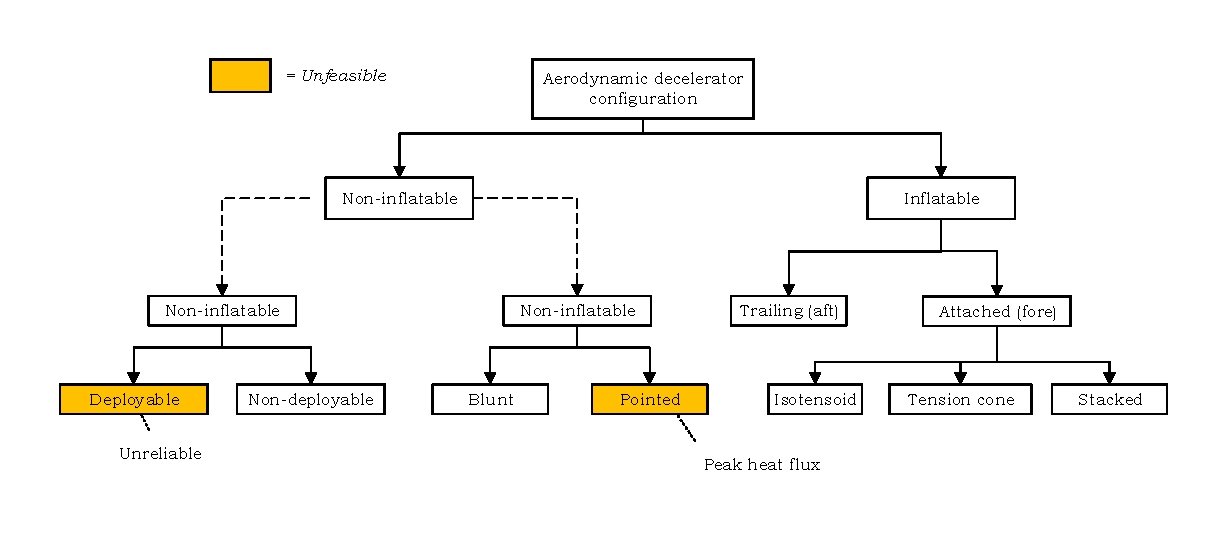
\includegraphics[width = 1.25\textwidth]{Figure/Concepts/DOT_configuration.pdf}
\vspace{-5mm}
\caption{\acrlong{dot} for entry vehicle configuration}
\label{fig:dotshape}
\end{figure}

Non-inflatable deployable concepts offer a lower reliability than and no particular advantages with respect to inflatable concepts and were therefore discarded. Pointed shapes were found infeasible by the peak heat flux generated. Lastly, combined inflatables were discarded since these add system complexity and mass while offering no additional advantages. 

Artist impressions of the resulting five concepts are given in Figure \ref{fig:concepts}. The concepts are:
\begin{itemize}
\item[(a)] A rigid concept, the conventional solution for re-entry. Its absence of deployment and its thereby limited diameter necessitates the use of a backshell to prevent the side of the payload capsule from excessive heating \cite{Hughes2005}.
\item[(b)] An isotensoid, a flexible bladder encapsulating the crew module that is inflated by ram-air through inlets mounted on it.
\item[(c)] A stacked toroid concept, in which multiple flexible rings are stacked on top of one another and inflated by an internal inflation system.
\item[(d)] A tension cone concept, which features one internally inflated torus and a flexible membrane that is spanned between the torus and the rigid centre body.
\item[(e)] A trailing ballute concept, the sole concept with a trailing inflatable. The inflated torus is connected to the payload capsule by a multitude of cables.
\end{itemize}

\begin{figure}[h]
	\centering
	\begin{subfigure}[b]{0.32\textwidth}
		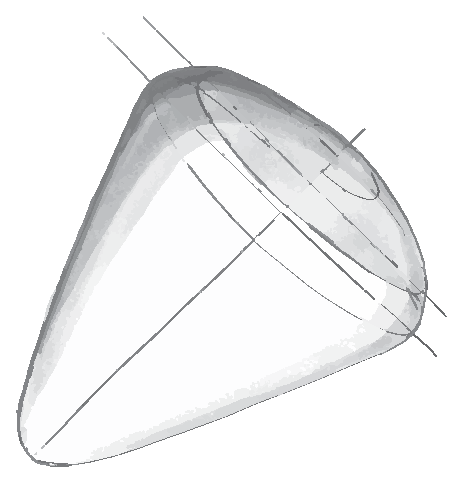
\includegraphics[angle=180, width=0.96\textwidth]{./Figure/Concepts/rigid.eps}
		\caption{Rigid concept}
		\label{fig:rigid}
	\end{subfigure}
	\begin{subfigure}[b]{0.32\textwidth}
		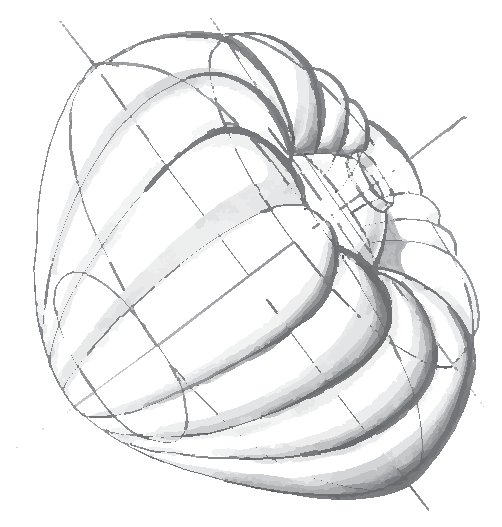
\includegraphics[width=0.96\textwidth]{./Figure/Concepts/isotensoid.eps}
		\caption{Isotensoid concept}
		\label{fig:isotensoid}
	\end{subfigure}
	\begin{subfigure}[b]{0.32\textwidth}
		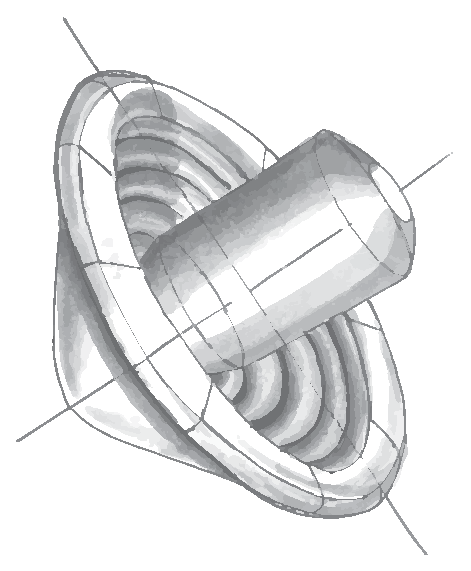
\includegraphics[width=0.96\textwidth]{./Figure/Concepts/stacked_toroid.eps}
		\caption{Stacked toroid concept}
		\label{fig:stacked_toroid}
	\end{subfigure}
	\begin{subfigure}[b]{0.32\textwidth}
		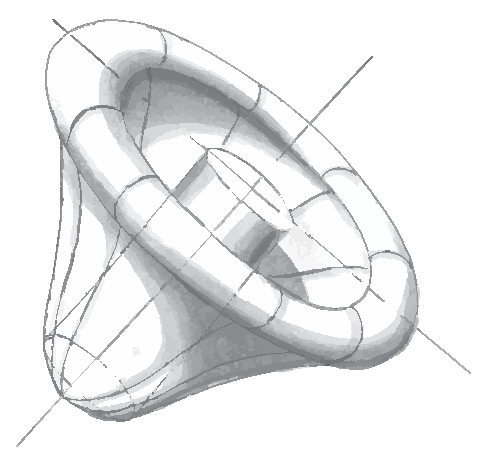
\includegraphics[width=0.96\textwidth]{./Figure/Concepts/tension_cone.eps}
		\caption{Tension cone concept}
		\label{fig:tension_cone}
	\end{subfigure}
	\begin{subfigure}[b]{0.32\textwidth}
		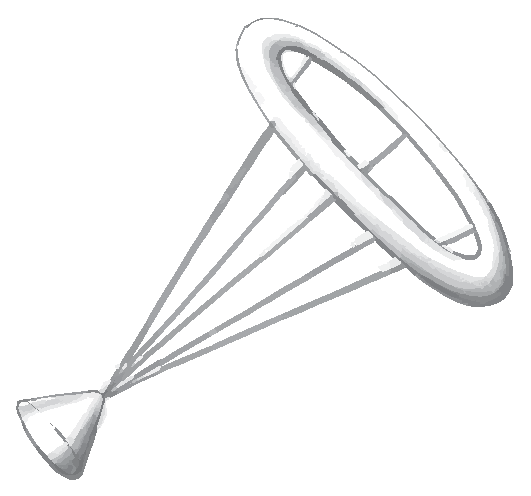
\includegraphics[width=0.96\textwidth]{./Figure/Concepts/trailing_ballute.eps}
		\caption{Trailing ballute concept}
		\label{fig:trailing_ballute}
	\end{subfigure}
\caption[Overview of design concepts]{Overview of design concepts (Courtesy of Irene Heemskerk)}
\label{fig:concepts}
\end{figure}






\subsection{Concept trade-off criteria} \label{sec:conceptcriteria}
Concepts have been evaluated on the basis of the following four criteria: decelerator mass, deceleration time, stability and development risk. These are discussed hereafter.

\subsubsection{Decelerator mass}
To take full advantage of launcher capability, the total vehicle mass is kept at its maximum. An increase in decelerator mass then leads to a decrease in payload mass, so it is essential that decelerator mass is kept to a minimum. To this end, the three primary components making up decelerator mass were evaluated for each concept: \gls{tps} mass, structural mass and control system mass. Their weighted average was computed to yield a total mass, taking into account their respective significance. The weight factors were determined from a comparable inflatable entry vehicle, namely \gls{irve} \cite{Hughes2005}.

The relative structural mass was determined using the structural mass estimation tool described in Section \ref{subsec:structool} and in more detail in the Mid-Term Report \cite[p.47-66]{Balasooriyan2015b}. Relative \gls{tps} mass is reflected by the estimated peak heat flux, a first-order estimation of the thermal energy to be dissipated and a key design driver for the \gls{tps}. Relative control system mass is reflected by the control moment required to be effected by the control system, in the form of the moment coefficient following from the aerodynamic analysis using modified Newtonian flow theory, as described in Section \ref{subsec:aerotool}. This was characterised by the lift-to-drag ratio, to account for the difference in lifting capability between concepts. Lower peak heat flux and low moment coefficients are favourable in terms of mass. 

\subsubsection{Deceleration time}
Minimising deceleration time is favourable for minimising ground operations expenses, since ground control is required to be fully active at the time of entry, which is the most critical mission phase. Furthermore, taxation of crew members is then alleviated. The time spent in the atmosphere is reflected by vehicle lift-to-drag ratio. For a given \gls{sym:CD}\gls{sym:A}, the maximum deceleration can be chosen by varying the lowest part of the trajectory: the density in lower parts of the atmosphere is higher, which then compensates for a low drag coefficient to produce the same force as a spacecraft with a high drag coefficient at a higher altitude with lower density. Because of the large variation of density in the atmosphere, it is possible to find a trajectory for any \gls{sym:CD}\gls{sym:A}. Thus, the drag coefficient itself is not a key driver for the design. However, the spacecraft can influence its deceleration time in the atmosphere by producing lift: if the spacecraft were to fly out of the atmosphere, a downward pointing lift would divert its trajectory more through the atmosphere. The ability of the spacecraft to influence this trajectory through the atmosphere is characterised by the amount of lift that can be produced, with respect to the amount of drag produced at the same \gls{sym:alpha}. The dependence on drag is due to the fact that two spacecraft with the same lift-to-drag ratio but a different \gls{sym:CD}\gls{sym:A}, will just have the lowest part of the trajectory at a different altitude, where the total lift and drag force will be the same for both spacecraft. Therefore, the deceleration time is characterised by the  lift-to-drag ratio. 

Lift and drag coefficients follow from the aerodynamic analysis tool, described in detail in the Mid-Term Report \cite[p.34-46]{Balasooriyan2015b}.

\subsubsection{Stability}
Vehicle stability is preferable, since a stable vehicle will react to disturbances with a restoring moment to revert to its original equilibrium condition without requiring control system activity. Not only does this reduce required control system activity, thereby limiting the system mass, but in addition the vehicle is more robust and less susceptible to perturbations. Stability is reflected by the static stability coefficient of concepts, following from aerodynamic analysis.

\subsubsection{Development risk}
It is key that concepts are evaluated for their development risk, an indication of schedule and cost risk. A concept with a high development risk will require extensive investigation to fully explore its capabilities and mitigate risks by technical uncertainty associated with such an underdeveloped concept. These investigation efforts incur additional cost and schedule risk. Development risk of concepts is evaluated by their \gls{trl}, denoting the current state of testing and application.





\subsection{Concept performance} \label{sec:conceptperf}
In terms of decelerator mass, the isotensoid was estimated to be the lightest concept, followed by the stacked toroid, illustrated in Table \ref{tab:cmass}. The tension cone and trailing ballute were notably heavier, primarily due to a higher structural mass. From this mass analysis, mass benefits of inflatable versus rigid concepts were clearly identifiable. On the basis of reference missions and scaling of estimated mechanical and thermal loading, decelerator thermo-structural mass was estimated at nearly 3000 $[kg]$. Key contributor was the backshell weighing well over 1400 $[kg]$. Such a backshell is not needed for the inflatable concepts. This mass was far in excess of the 1000 $[kg]$ limit imposed on maximum decelerator mass.

\begin{table}[h]
\centering
\caption[Concept mass comparison]{Concept mass comparison (expressed as percentage of stacked toroid mass)}\label{tab:cmass}
\begin{tabular}{|p{0.2\textwidth}|p{0.2\textwidth}|p{0.2\textwidth}|p{0.2\textwidth}||p{0.079\textwidth}|}

\hline
                          & \textbf{Structural mass (20\%)} & \textbf{Thermal mass (50\%)} & \textbf{Control system mass (15\%)} & \textbf{Total mass} \\ \hline
\textbf{Stacked toroid}   &  100                                 & 100                          & 100                                      &\cellcolor{green!70}  100                           \\ \hline
\textbf{Tension cone}     &  168                               & 100                               &  100                                     &\cellcolor{yellow!70} 116                                 \\ \hline
\textbf{Trailing ballute} &  221                                 & 84                               & 67                                      &\cellcolor{yellow!70} 113 \\ \hline
\textbf{Isotensoid}       &  110                                 & 76                               & 96                                      &\cellcolor{green!70} 88 \\ \hline \hline
\textbf{Rigid}            &  \multicolumn{4}{|p{0.762\textwidth}|}{\cellcolor{red!60} ~~~~~~~~~~~Estimated 3000 $[kg]$: Far in excess of 1000 $[kg]$ limit}    \\ \hline
\end{tabular}
\end{table}

In terms of deceleration time, lift-to-drag ratio, performance of the rigid concept was best, that of the isotensoid notably worst and those of the other three inflatable concepts in between and comparable. In terms of concept static stability, the isotensoid again performed notably worst, being unstable. The rigid concept proved neutrally stable and the other three inflatables are stable. These results are illustrated by Tables \ref{tab:decel} and \ref{tab:stab}.

\begin{table}[h]
\caption{Review of concept deceleration time}
%\hspace{-10mm}
\centering
\begin{tabular}{|p{0.2\textwidth}|p{0.12\textwidth}|p{0.12\textwidth}|p{0.12\textwidth}|p{0.12\textwidth}|p{0.12\textwidth}|}
\hline
\textbf{}                          & \textbf{Stacked toroid} & \textbf{Tension cone} & \textbf{Trailing ballute} & \textbf{Isotensoid} & \textbf{Rigid} \\ \hline
\textbf{Lift-to-drag ratio} & \cellcolor{yellow!75} -0.176  &\cellcolor{yellow!75} -0.176   &\cellcolor{yellow!75} -0.210 & \cellcolor{red!60} -0.072 &\cellcolor{green!70} -0.311              \\ \hline
\textbf{Deceleration performance} &\cellcolor{yellow!75} Adequate &\cellcolor{yellow!75}  Adequate  &\cellcolor{yellow!75} Adequate & \cellcolor{red!60}     Poor       &\cellcolor{green!70} Excellent                 \\ \hline
\end{tabular}
\label{tab:decel}
\end{table}

\begin{table}[h]
\caption{Review of concept stability}
%\hspace{-10mm}
\centering
\begin{tabular}{|p{0.2\textwidth}|p{0.12\textwidth}|p{0.12\textwidth}|p{0.12\textwidth}|p{0.12\textwidth}|p{0.12\textwidth}|}
\hline
\textbf{}                          & \textbf{Stacked toroid} & \textbf{Tension cone} & \textbf{Trailing ballute} & \textbf{Isotensoid} & \textbf{Rigid} \\ \hline
\textbf{Static stability} &\cellcolor{green!70} Stable  &\cellcolor{green!70}  Stable   &\cellcolor{green!70} Stable & \cellcolor{red!60}   Unstable          &\cellcolor{yellow!75} Neutrally stable                 \\ \hline
\end{tabular}
\label{tab:stab}
\end{table}

Technology readiness, reflected by the \glspl{trl} in Table \ref{tab:gls_rev}, is highest for the conventionally tested and flown rigid concept. The stacked toroid concept was flown in multiple NASA (\gls{irve}) missions and prototypes thereof have thus been tested in a relevant environment. The other three inflatables have received notably less attention, having solely undergone wind tunnel and laboratory testing. In addition, the difficulty of controlling a trailing ballute using conventional methods necessitates the use of morphing. As morphing is a relatively underdeveloped concept and has only been formulated in theory for trailing ballute configurations, the \gls{trl} of the trailing ballute reflects this by being the lowest.

\begin{table}[h]
\centering
\caption{Review of concept development risk}
\begin{tabular}{|p{0.2\textwidth}|p{0.12\textwidth}|p{0.12\textwidth}|p{0.12\textwidth}|p{0.12\textwidth}|p{0.12\textwidth}|}
\hline
\textbf{Concept {[}-{]}} & \textbf{Stacked toroid} & \textbf{Tension cone} & \textbf{Trailing ballute} & \textbf{Isotensoid} & \textbf{Rigid} \\ \hline \hline
\textbf{TRL {[}-{]}}     &\cellcolor{green!70} 7  &\cellcolor{yellow!75}  4   &\cellcolor{red!60} 2 & \cellcolor{yellow!75}      4          &\cellcolor{green!70} 9     \\ \hline
\end{tabular}
\label{tab:gls_rev}
\end{table}










